\chapter{Expérimentations}
\section{Données}
\paragraph{}
Les données de tests sont les même vues dans \ref{part1}\ref{dataSet}, ici nous traiterons uniquement les instances satisfiables (uf75-325).

\section{Machines}
\paragraph{}Les machines sont les mêmes que celles utilisées dans \ref{machines} pour rester consistant et faire une comparaison cohérente entres les résultats.
\section{Résultats}
\subsection{ACS}
\paragraph{}\label{testconds}
Les conditions de test restent inchangées, autrement dit : \\
Dix essaies par instance pour dix instances en faisant varier les paramètres empiriques à l'exception de $\rho$ le taux d'évaporation fixé à 0.7 pour chaque test : 
\paragraph{Remarque} : la version d'ACS est celle avec les actions \textbf{deamons} vus dans \ref{deamons}.
\begin{table}[H]
	\centering
	\resizebox{\textwidth}{!}{%
		\begin{tabular}{|c|c|c|c|c|c|c|c|c|}
			\hline
			\textbf{maxItter} & \textbf{maxStep} & \textbf{Nbr. fourmis} & \textbf{alpha} & \textbf{beta} & \textbf{q$_{\text{\textbf{0}}}$} & \textbf{Moyenne} & \textbf{Taux moy.} & \textbf{Temps moy(s)} \\ \hline
			500               & 30               & 30                       & 0.8            & 0.3           & 0.6        & 324.7            & 0.9990769231       & 2.51844               \\ \hline
			500               & 30               & 30                       & 1              & 0             & 0.6        & 324.66           & 0.9989538462       & 2.55154               \\ \hline
			500               & 25               & 30                       & 0.8            & 0             & 0.6        & 324.65           & 0.9989230769       & 2.30747               \\ \hline
			500               & 25               & 30                       & 0.8            & 0.3           & 0.6        & 324.64           & 0.9988923077       & 2.22491               \\ \hline
			500               & 30               & 30                       & 1              & 0.3           & 0.6        & 324.6            & 0.9987692308       & 2.47566               \\ \hline
			500               & 25               & 30                       & 1              & 0             & 0.6        & 324.57           & 0.9986769231       & 2.28502               \\ \hline
		\end{tabular}%
	}
	\caption{Meilleurs jeux de paramètres pour l'ensemble des instances choisies (ACS)}
\end{table}
\newpage
\subsection{AS}
\paragraph{}
Les conditions restent inchangées.

% Please add the following required packages to your document preamble:
% \usepackage{graphicx}
\begin{table}[H]
	\centering
	\resizebox{\textwidth}{!}{%
		\begin{tabular}{|c|c|c|c|c|c|c|c|}
		\hline
		\textbf{maxItter} & \textbf{maxStep} & \textbf{Nbr. fourmis} & \textbf{alpha} & \textbf{beta} & \textbf{Moy. Sat} & \textbf{Taux moy.} & \textbf{Temps moy(s)} \\ \hline
			100 & 30 & 30 & 1   & 0.3 & 323.75 & 0.9961538462 & 0.52013 \\ \hline
			100 & 25 & 30 & 1   & 0.3 & 323.67 & 0.9959076923 & 0.45238 \\ \hline
			500 & 30 & 30 & 1   & 0   & 323.65 & 0.9958461538 & 2.50055 \\ \hline
			100 & 30 & 30 & 0.8 & 0   & 323.65 & 0.9958461538 & 0.56023 \\ \hline
			500 & 25 & 30 & 0.8 & 0   & 323.64 & 0.9958153846 & 2.0897  \\ \hline
			100 & 25 & 30 & 0.8 & 0.3 & 323.61 & 0.9957230769 & 0.43755 \\ \hline
		\end{tabular}%
	}
		\caption{Meilleurs jeux de paramètres pour l'ensemble des instances choisies (AS)}
\end{table}

\section{Comparaison entre AS et ACS}
\paragraph{}
Le graphe suivant compare les taux de satisfiabilité moyens des trois meilleurs jeux de paramètres pour AS et ACS : \\

\begin{figure}[H]
	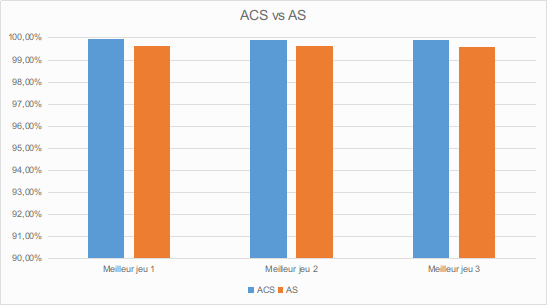
\includegraphics[width=\textwidth]{images/acsVSas.png}
\end{figure}

\paragraph{}
Comme le prévoyait l'aspect théorique, ACS est nettement supérieure en terme de taux de satisfiabilité à son homologue AS, cela est dû principalement au fait que ce dernier n'est pas une représentation fidèle  du comportement réel des fourmis, contrairement à ACS qui, par le bias de la marche aléatoire, se veut plus réaliste et représentatif de la vie réelle. bien que la différence est négligeable, cela reste une comparaison a petite échelle, dans les cas réels les instances sont beaucoup plus complexes et difficiles à résoudre.
%talk about how BSO is amazing
